% Generated by Sphinx.
\def\sphinxdocclass{report}
\documentclass[letterpaper,10pt,openany,oneside]{sphinxmanual}
\usepackage[utf8]{inputenc}
\DeclareUnicodeCharacter{00A0}{\nobreakspace}
\usepackage[T1]{fontenc}
\usepackage[english]{babel}
\usepackage{times}
\usepackage[Bjarne]{fncychap}
\usepackage{longtable}
\usepackage{sphinx}
\usepackage{multirow}
\usepackage{booktabs}
\usepackage{array}
\definecolor{nrelblue}{RGB}{0, 121, 193}
\hypersetup{linkcolor=nrelblue}
\usepackage[section]{placeins}


\title{csm Documentation}
\date{June 19, 2013}
\release{0.1.0}
\author{George Scott and Katherine Dykes}
\newcommand{\sphinxlogo}{}
\renewcommand{\releasename}{Release}
\makeindex

\makeatletter
\def\PYG@reset{\let\PYG@it=\relax \let\PYG@bf=\relax%
    \let\PYG@ul=\relax \let\PYG@tc=\relax%
    \let\PYG@bc=\relax \let\PYG@ff=\relax}
\def\PYG@tok#1{\csname PYG@tok@#1\endcsname}
\def\PYG@toks#1+{\ifx\relax#1\empty\else%
    \PYG@tok{#1}\expandafter\PYG@toks\fi}
\def\PYG@do#1{\PYG@bc{\PYG@tc{\PYG@ul{%
    \PYG@it{\PYG@bf{\PYG@ff{#1}}}}}}}
\def\PYG#1#2{\PYG@reset\PYG@toks#1+\relax+\PYG@do{#2}}

\def\PYG@tok@gd{\def\PYG@tc##1{\textcolor[rgb]{0.63,0.00,0.00}{##1}}}
\def\PYG@tok@gu{\let\PYG@bf=\textbf\def\PYG@tc##1{\textcolor[rgb]{0.50,0.00,0.50}{##1}}}
\def\PYG@tok@gt{\def\PYG@tc##1{\textcolor[rgb]{0.00,0.25,0.82}{##1}}}
\def\PYG@tok@gs{\let\PYG@bf=\textbf}
\def\PYG@tok@gr{\def\PYG@tc##1{\textcolor[rgb]{1.00,0.00,0.00}{##1}}}
\def\PYG@tok@cm{\let\PYG@it=\textit\def\PYG@tc##1{\textcolor[rgb]{0.25,0.50,0.56}{##1}}}
\def\PYG@tok@vg{\def\PYG@tc##1{\textcolor[rgb]{0.73,0.38,0.84}{##1}}}
\def\PYG@tok@m{\def\PYG@tc##1{\textcolor[rgb]{0.13,0.50,0.31}{##1}}}
\def\PYG@tok@mh{\def\PYG@tc##1{\textcolor[rgb]{0.13,0.50,0.31}{##1}}}
\def\PYG@tok@cs{\def\PYG@tc##1{\textcolor[rgb]{0.25,0.50,0.56}{##1}}\def\PYG@bc##1{\colorbox[rgb]{1.00,0.94,0.94}{##1}}}
\def\PYG@tok@ge{\let\PYG@it=\textit}
\def\PYG@tok@vc{\def\PYG@tc##1{\textcolor[rgb]{0.73,0.38,0.84}{##1}}}
\def\PYG@tok@il{\def\PYG@tc##1{\textcolor[rgb]{0.13,0.50,0.31}{##1}}}
\def\PYG@tok@go{\def\PYG@tc##1{\textcolor[rgb]{0.19,0.19,0.19}{##1}}}
\def\PYG@tok@cp{\def\PYG@tc##1{\textcolor[rgb]{0.00,0.44,0.13}{##1}}}
\def\PYG@tok@gi{\def\PYG@tc##1{\textcolor[rgb]{0.00,0.63,0.00}{##1}}}
\def\PYG@tok@gh{\let\PYG@bf=\textbf\def\PYG@tc##1{\textcolor[rgb]{0.00,0.00,0.50}{##1}}}
\def\PYG@tok@ni{\let\PYG@bf=\textbf\def\PYG@tc##1{\textcolor[rgb]{0.84,0.33,0.22}{##1}}}
\def\PYG@tok@nl{\let\PYG@bf=\textbf\def\PYG@tc##1{\textcolor[rgb]{0.00,0.13,0.44}{##1}}}
\def\PYG@tok@nn{\let\PYG@bf=\textbf\def\PYG@tc##1{\textcolor[rgb]{0.05,0.52,0.71}{##1}}}
\def\PYG@tok@no{\def\PYG@tc##1{\textcolor[rgb]{0.38,0.68,0.84}{##1}}}
\def\PYG@tok@na{\def\PYG@tc##1{\textcolor[rgb]{0.25,0.44,0.63}{##1}}}
\def\PYG@tok@nb{\def\PYG@tc##1{\textcolor[rgb]{0.00,0.44,0.13}{##1}}}
\def\PYG@tok@nc{\let\PYG@bf=\textbf\def\PYG@tc##1{\textcolor[rgb]{0.05,0.52,0.71}{##1}}}
\def\PYG@tok@nd{\let\PYG@bf=\textbf\def\PYG@tc##1{\textcolor[rgb]{0.33,0.33,0.33}{##1}}}
\def\PYG@tok@ne{\def\PYG@tc##1{\textcolor[rgb]{0.00,0.44,0.13}{##1}}}
\def\PYG@tok@nf{\def\PYG@tc##1{\textcolor[rgb]{0.02,0.16,0.49}{##1}}}
\def\PYG@tok@si{\let\PYG@it=\textit\def\PYG@tc##1{\textcolor[rgb]{0.44,0.63,0.82}{##1}}}
\def\PYG@tok@s2{\def\PYG@tc##1{\textcolor[rgb]{0.25,0.44,0.63}{##1}}}
\def\PYG@tok@vi{\def\PYG@tc##1{\textcolor[rgb]{0.73,0.38,0.84}{##1}}}
\def\PYG@tok@nt{\let\PYG@bf=\textbf\def\PYG@tc##1{\textcolor[rgb]{0.02,0.16,0.45}{##1}}}
\def\PYG@tok@nv{\def\PYG@tc##1{\textcolor[rgb]{0.73,0.38,0.84}{##1}}}
\def\PYG@tok@s1{\def\PYG@tc##1{\textcolor[rgb]{0.25,0.44,0.63}{##1}}}
\def\PYG@tok@gp{\let\PYG@bf=\textbf\def\PYG@tc##1{\textcolor[rgb]{0.78,0.36,0.04}{##1}}}
\def\PYG@tok@sh{\def\PYG@tc##1{\textcolor[rgb]{0.25,0.44,0.63}{##1}}}
\def\PYG@tok@ow{\let\PYG@bf=\textbf\def\PYG@tc##1{\textcolor[rgb]{0.00,0.44,0.13}{##1}}}
\def\PYG@tok@sx{\def\PYG@tc##1{\textcolor[rgb]{0.78,0.36,0.04}{##1}}}
\def\PYG@tok@bp{\def\PYG@tc##1{\textcolor[rgb]{0.00,0.44,0.13}{##1}}}
\def\PYG@tok@c1{\let\PYG@it=\textit\def\PYG@tc##1{\textcolor[rgb]{0.25,0.50,0.56}{##1}}}
\def\PYG@tok@kc{\let\PYG@bf=\textbf\def\PYG@tc##1{\textcolor[rgb]{0.00,0.44,0.13}{##1}}}
\def\PYG@tok@c{\let\PYG@it=\textit\def\PYG@tc##1{\textcolor[rgb]{0.25,0.50,0.56}{##1}}}
\def\PYG@tok@mf{\def\PYG@tc##1{\textcolor[rgb]{0.13,0.50,0.31}{##1}}}
\def\PYG@tok@err{\def\PYG@bc##1{\fcolorbox[rgb]{1.00,0.00,0.00}{1,1,1}{##1}}}
\def\PYG@tok@kd{\let\PYG@bf=\textbf\def\PYG@tc##1{\textcolor[rgb]{0.00,0.44,0.13}{##1}}}
\def\PYG@tok@ss{\def\PYG@tc##1{\textcolor[rgb]{0.32,0.47,0.09}{##1}}}
\def\PYG@tok@sr{\def\PYG@tc##1{\textcolor[rgb]{0.14,0.33,0.53}{##1}}}
\def\PYG@tok@mo{\def\PYG@tc##1{\textcolor[rgb]{0.13,0.50,0.31}{##1}}}
\def\PYG@tok@mi{\def\PYG@tc##1{\textcolor[rgb]{0.13,0.50,0.31}{##1}}}
\def\PYG@tok@kn{\let\PYG@bf=\textbf\def\PYG@tc##1{\textcolor[rgb]{0.00,0.44,0.13}{##1}}}
\def\PYG@tok@o{\def\PYG@tc##1{\textcolor[rgb]{0.40,0.40,0.40}{##1}}}
\def\PYG@tok@kr{\let\PYG@bf=\textbf\def\PYG@tc##1{\textcolor[rgb]{0.00,0.44,0.13}{##1}}}
\def\PYG@tok@s{\def\PYG@tc##1{\textcolor[rgb]{0.25,0.44,0.63}{##1}}}
\def\PYG@tok@kp{\def\PYG@tc##1{\textcolor[rgb]{0.00,0.44,0.13}{##1}}}
\def\PYG@tok@w{\def\PYG@tc##1{\textcolor[rgb]{0.73,0.73,0.73}{##1}}}
\def\PYG@tok@kt{\def\PYG@tc##1{\textcolor[rgb]{0.56,0.13,0.00}{##1}}}
\def\PYG@tok@sc{\def\PYG@tc##1{\textcolor[rgb]{0.25,0.44,0.63}{##1}}}
\def\PYG@tok@sb{\def\PYG@tc##1{\textcolor[rgb]{0.25,0.44,0.63}{##1}}}
\def\PYG@tok@k{\let\PYG@bf=\textbf\def\PYG@tc##1{\textcolor[rgb]{0.00,0.44,0.13}{##1}}}
\def\PYG@tok@se{\let\PYG@bf=\textbf\def\PYG@tc##1{\textcolor[rgb]{0.25,0.44,0.63}{##1}}}
\def\PYG@tok@sd{\let\PYG@it=\textit\def\PYG@tc##1{\textcolor[rgb]{0.25,0.44,0.63}{##1}}}

\def\PYGZbs{\char`\\}
\def\PYGZus{\char`\_}
\def\PYGZob{\char`\{}
\def\PYGZcb{\char`\}}
\def\PYGZca{\char`\^}
% for compatibility with earlier versions
\def\PYGZat{@}
\def\PYGZlb{[}
\def\PYGZrb{]}
\makeatother

\begin{document}

\maketitle
\tableofcontents
\phantomsection\label{index::doc}



\chapter{Introduction}
\label{intro:code-name}\label{intro:introduction}\label{intro::doc}
The set of models contained in this software allow for the determination of wind plant cost of energy including models for turbine capital costs, balance of station costs, operations and maintenance costs, and annual energy production.  It is a direct implementation of the model described in {[}Fingersh2006{]} with modifications as described in {[}Maples2010{]}.


\chapter{Installation}
\label{installation:installation}\label{installation::doc}
\begin{notice}{note}{prerequisites}

NumPy, SciPy
\end{notice}

Download either csm.py-0.1.0.tar.gz or csm.py-0.1.0.zip, and uncompress/unpack it.

Install HubNacelleCST with the following command.

\begin{quote}
\begin{Verbatim}[commandchars=\\\{\}]
\PYG{n+nv}{\$ }python setup.py install
\end{Verbatim}
\end{quote}

To check if installation was successful run the unit tests for the NREL 5MW model

\begin{quote}
\begin{Verbatim}[commandchars=\\\{\}]
\PYG{n+nv}{\$ }python \PYG{n+nb}{test}/test\PYGZus{}csm.py
\end{Verbatim}
\end{quote}

An `OK' signifies that all the tests passed.

To access an HTML version of this documentation which contains further details and links to the source code, open docs/index.html.


\chapter{Tutorial}
\label{tutorial:tutorial-label}\label{tutorial::doc}\label{tutorial:tutorial}
To be done...


\chapter{Module Documentation}
\label{documentation::doc}\label{documentation:module-documentation}
To be done...


\section{Cost and Scaling Model Utilities}
\label{documentation:cost-and-scaling-model-utilities}
Cost escalators are used to adjust for input factor prices trends for materials and labor associated with turbine manufacturing, plant development and operation.


\section{Turbine Capital Costs (TCC) Module}
\label{documentation:turbine-capital-costs-tcc-module}\phantomsection\label{documentation:module-csm.src.csmTurbine}\index{csm.src.csmTurbine (module)}
The NREL Cost and Scaling Model turbine module calculates turbine component costs and masses (either onshore or offshore).  This excludes the foundation which is considered part of the balance of station even for offshore plants.


\subsection{csmTurbine}
\label{documentation:csmturbine}
This class calculates the the component masses and costs for a wind turbine using the NREL Cost and Scaling Model.
\index{csmTurbine (class in csm.src.csmTurbine)}

\begin{fulllineitems}
\phantomsection\label{documentation:csm.src.csmTurbine.csmTurbine}\pysigline{\strong{class }\code{csm.src.csmTurbine.}\bfcode{csmTurbine}}
\end{fulllineitems}


\textbf{Methods}

\begin{tabular}{>{\raggedright\arraybackslash}p{0.42\textwidth}@{\qquad}p{0.45\textwidth}}\toprule

\code{\_\_init\_\_}()
 & 
Initialize properties for operations and maintenance costs.
\\\midrule

\code{compute}({[}hubHeight, machineRating, ...{]})
 & 
Computes the turbine component masses and costs using the NREL Cost and Scaling Model method.
\\\midrule

\code{getMass}()
 & 
Provides the overall turbine mass.
\\\midrule

\code{getCost}()
 & 
Provides the turbine capital costs for a single turbine.
\\\bottomrule
\end{tabular}


There are several sub-modules in the overall TCC module for each of the major sub-systems including the blades, hub, nacelle and tower.


\subsection{csmBlades}
\label{documentation:csmblades}
This class calculates wind turbine blade mass and cost based on the NREL Cost and Scaling Model.
\index{csmBlades (class in csm.src.csmBlades)}

\begin{fulllineitems}
\phantomsection\label{documentation:csm.src.csmBlades.csmBlades}\pysigline{\strong{class }\code{csm.src.csmBlades.}\bfcode{csmBlades}}
\end{fulllineitems}


\textbf{Methods}

\begin{tabular}{>{\raggedright\arraybackslash}p{0.42\textwidth}@{\qquad}p{0.45\textwidth}}\toprule

\code{\_\_init\_\_}()
 & 
Initialize the parameters for the wind turbine blade
\\\midrule

\code{compute}({[}diam, advanced, curr\_yr, curr\_mon, ...{]})
 & 
Compute mass and cost for a single wind turbine blade by calling computeMass and computeCost
\\\midrule

\code{computeMass}(diam{[}, advanced{]})
 & 
Compute mass for a single wind turbine blade using NREL cost and scaling model
\\\midrule

\code{computeCost}(diam{[}, advanced, curr\_yr, curr\_mon{]})
 & 
Compute cost for a single wind turbine blade using NREL cost and scaling model
\\\midrule

\code{getMass}()
 & 
Provides the mass for the wind turbine blade.
\\\midrule

\code{getCost}()
 & 
Provides the cost for the wind turbine blade.
\\\bottomrule
\end{tabular}


\textbf{Example}

The following is an example use of the individual csmBlades module.

Output should be:

Conventional blade design:
Blades    276129.6 K\$   25614.4 kg

Advanced blade design:
Blades    251227.0 K\$   17650.7 kg


\subsection{csmHub}
\label{documentation:csmhub}
This class calculates wind turbine hub system mass and cost based on the NREL Cost and Scaling Model.
\index{csmHub (class in csm.src.csmHub)}

\begin{fulllineitems}
\phantomsection\label{documentation:csm.src.csmHub.csmHub}\pysigline{\strong{class }\code{csm.src.csmHub.}\bfcode{csmHub}}
\end{fulllineitems}


\textbf{Methods}

\begin{tabular}{>{\raggedright\arraybackslash}p{0.42\textwidth}@{\qquad}p{0.45\textwidth}}\toprule

\code{\_\_init\_\_}()
 & 
Initialize the parameters for csm Hub
\\\midrule

\code{compute}(blademass{[}, diam, nblades, curr\_yr, ...{]})
 & 
Compute mass and cost for the hub system by calling computeMass and computeCost
\\\midrule

\code{computeMass}(blademass{[}, diam, nblades{]})
 & 
Compute mass for the hub system based on NREL Cost and Scaling Model
\\\midrule

\code{computeCost}({[}diam, curr\_yr, curr\_mon, ...{]})
 & 
Compute cost for the hub system by the NREL Cost and Scaling Model
\\\midrule

\code{getMass}()
 & 
Provides the overall hub system mass.
\\\midrule

\code{getCost}()
 & 
Provides the overall hub system cost.
\\\midrule

\code{getHubComponentMasses}()
 & 
Provides the detail on hub system component masses.
\\\midrule

\code{getHubComponentCosts}()
 & 
Provides the overall hub system cost.
\\\bottomrule
\end{tabular}


\textbf{Example}

The following is an example use of the individual csmHub module.

The output should be:
\begin{description}
\item[{Hub System Components:}] \leavevmode\\
Hub     124903.9 K\$  22519.7 kg
Pitch Mech   24379.7 K\$  10313.9 kg
Nose Cone   10509.0 K\$  1810.5 kg

\end{description}

Hub total   379152.6 K\$  34644.2 kg


\subsection{csmNacelle}
\label{documentation:csmnacelle}
This class calculates wind turbine hub system mass and cost based on the NREL Cost and Scaling Model.
\index{csmNacelle (class in csm.src.csmNacelle)}

\begin{fulllineitems}
\phantomsection\label{documentation:csm.src.csmNacelle.csmNacelle}\pysigline{\strong{class }\code{csm.src.csmNacelle.}\bfcode{csmNacelle}}
\end{fulllineitems}


\textbf{Methods}

\begin{tabular}{>{\raggedright\arraybackslash}p{0.42\textwidth}@{\qquad}p{0.45\textwidth}}\toprule

\code{\_\_init\_\_}()
 & 
Initialize the parameters for the nacelle
\\\midrule

\code{compute}(RotorDiam, MachineRating, RotorMass, ...)
 & 
Compute mass and cost for a full wind turbine Nacelle by calling computeMass and computeCost
\\\midrule

\code{computeMass}(RotorDiam, MachineRating, ...{[}, ...{]})
 & 
Compute mass for a full wind turbine Nacelle using the NREL Cost and Scaling Model
\\\midrule

\code{computeCost}(RotorDiam, MachineRating, ...{[}, ...{]})
 & 
Compute cost for a full wind turbine Nacelle using the NREL Cost and Scaling Model
\\\midrule

\code{getMass}()
 & 
Provides the mass for the overall wind turbine nacelle assembly.
\\\midrule

\code{getCost}()
 & 
Provides the cost for the overall wind turbine nacelle assembly.
\\\midrule

\code{getNacelleComponentMasses}()
 & 
Provides the mass for the overall wind turbine nacelle components.
\\\midrule

\code{getNacelleComponentCosts}()
 & 
Provides the cost for the overall wind turbine nacelle components.
\\\bottomrule
\end{tabular}


\textbf{Example}

The following is an example use of the individual csmNacelle module.

Output should be:

Nacelle Total  3249404.5229 K\$  223315.6984 kg

Within the nacelle, there are additional sub-modules for the low-speed shaft, the gearbox and the generator.


\subsection{LowSpdShaft}
\label{documentation:lowspdshaft}
This class calculates wind turbine low speed shaft mass and cost based on the NREL Cost and Scaling Model.
\index{LowSpdShaft (class in csm.src.csmNacelle)}

\begin{fulllineitems}
\phantomsection\label{documentation:csm.src.csmNacelle.LowSpdShaft}\pysigline{\strong{class }\code{csm.src.csmNacelle.}\bfcode{LowSpdShaft}}
\end{fulllineitems}


\textbf{Methods}

\begin{tabular}{>{\raggedright\arraybackslash}p{0.42\textwidth}@{\qquad}p{0.45\textwidth}}\toprule

\code{\_\_init\_\_}()
 & 
Initialize the parameters for low speed shaft
\\\midrule

\code{compute}(RotorDiam, RotorMass, RotorTorque, ...)
 & 
Compute mass and cost for a low speed shaft by calling computeMass and computeCost
\\\midrule

\code{computeMass}(RotorDiam, RotorMass, RotorTorque)
 & 
Compute mass for a low speed shaft using the NREL Cost and Scaling Model
\\\midrule

\code{computeCost}(RotorDiam, curr\_yr, curr\_mon)
 & 
Compute cost for a low speed shaft using the NREL Cost and Scaling Model
\\\midrule

\code{getMass}()
 & 
Provides the mass for the low speed shaft.
\\\midrule

\code{getCost}()
 & 
Provides the cost for the wind turbine low speed shaft.
\\\bottomrule
\end{tabular}



\subsection{GearBox}
\label{documentation:gearbox}
This class calculates wind turbine gearbox mass and cost based on the NREL Cost and Scaling Model.
\index{GearBox (class in csm.src.csmNacelle)}

\begin{fulllineitems}
\phantomsection\label{documentation:csm.src.csmNacelle.GearBox}\pysigline{\strong{class }\code{csm.src.csmNacelle.}\bfcode{GearBox}}
\end{fulllineitems}


\textbf{Methods}

\begin{tabular}{>{\raggedright\arraybackslash}p{0.42\textwidth}@{\qquad}p{0.45\textwidth}}\toprule

\code{\_\_init\_\_}()
 & 
Initialize the parameters for gearbox
\\\midrule

\code{compute}(iDsgn, MachineRating, RotorTorque, ...)
 & 
Compute mass and cost for a gearbox by calling computeMass and computeCost
\\\midrule

\code{computeMass}(iDsgn, RotorTorque)
 & 
Compute mass for a gearbox using the cost and scaling model
\\\midrule

\code{computeCost}(iDsgn, MachineRating, curr\_yr, ...)
 & 
Compute cost for a gearbox using the NREL Cost and Scaling Model
\\\midrule

\code{getMass}()
 & 
Provides the mass for the gearbox.
\\\midrule

\code{getCost}()
 & 
Provides the cost for the wind turbine gearbox.
\\\bottomrule
\end{tabular}



\subsection{Generator}
\label{documentation:generator}
This class calculates wind turbine generator mass and cost based on the NREL Cost and Scaling Model.
\index{Generator (class in csm.src.csmNacelle)}

\begin{fulllineitems}
\phantomsection\label{documentation:csm.src.csmNacelle.Generator}\pysigline{\strong{class }\code{csm.src.csmNacelle.}\bfcode{Generator}}
\end{fulllineitems}


\textbf{Methods}

\begin{tabular}{>{\raggedright\arraybackslash}p{0.42\textwidth}@{\qquad}p{0.45\textwidth}}\toprule

\code{\_\_init\_\_}()
 & 
Initialize the parameters for the generator
\\\midrule

\code{compute}(iDsgn, MachineRating, RotorTorque, ...)
 & 
Compute mass and cost for a generator by calling computeMass and computeCost
\\\midrule

\code{computeMass}(iDsgn, MachineRating, RotorTorque)
 & 
Compute mass for a generator using the NREL Cost and Scaling Model
\\\midrule

\code{computeCost}(iDsgn, MachineRating, curr\_yr, ...)
 & 
Compute mass and cost for a generator using the NREL Cost and Scaling Model
\\\midrule

\code{getMass}()
 & 
Provides the mass for the generator.
\\\midrule

\code{getCost}()
 & 
Provides the cost for the wind turbine generator.
\\\bottomrule
\end{tabular}



\subsection{csmTower}
\label{documentation:csmtower}
This class calculates wind turbine tower mass and cost based on the NREL Cost and Scaling Model.
\index{csmTower (class in csm.src.csmTower)}

\begin{fulllineitems}
\phantomsection\label{documentation:csm.src.csmTower.csmTower}\pysigline{\strong{class }\code{csm.src.csmTower.}\bfcode{csmTower}}
\end{fulllineitems}


\textbf{Methods}

\begin{tabular}{>{\raggedright\arraybackslash}p{0.42\textwidth}@{\qquad}p{0.45\textwidth}}\toprule

\code{\_\_init\_\_}()
 & 
Initialize the parameters for the wind turbine tower
\\\midrule

\code{compute}(RotorDiam, HubHeight{[}, curr\_yr, ...{]})
 & 
Compute mass and cost for a wind turbine tower by calling computeMass and computeCost
\\\midrule

\code{computeMass}(RotorDiam, HubHeight)
 & 
Compute mass for a wind turbine tower using the NREL Cost and Scaling Model
\\\midrule

\code{computeCost}(curr\_yr, curr\_mon{[}, towerMass{]})
 & 
Compute cost for a wind turbine tower by calling computeMass and computeCost
\\\midrule

\code{getMass}()
 & 
Provides the mass for the wind turbine tower.
\\\midrule

\code{getCost}()
 & 
Provides the cost for the wind turbine tower.
\\\bottomrule
\end{tabular}


\textbf{Example}

The following is an example use of the individual csmTower module.

Output should be:

Tower Mass: 444384.157764
Tower Cost: 1009500.23594

\textbf{Examples}
The following is an example use of the overall csmTurbine module for calculating the onshore and offshore wind turbine costs using the NREL 5 MW reference turbine {\color{red}\bfseries{}{[}1{]}\_}:

Output should be:

Onshore configuration 5 MW turbine:
Turbine total: 5487334.85 \$K  774049.19 kg

Offshore configuration 5 MW turbine:
Turbine total: 6064385.11 \$K  774049.19 kg

\textbf{References}


\section{Balance of Station Costs (BOS) Module}
\label{documentation:balance-of-station-costs-bos-module}\phantomsection\label{documentation:module-csm.src.csmBOS}\index{csm.src.csmBOS (module)}
The NREL Cost and Scaling Model balance of station module calculates the installation, assembly and other non-turbine capital costs associated with the development of a wind plant (either onshore or offshore).  The foundation is considered part of the balance of station even for offshore plants.


\subsection{csmBOS}
\label{documentation:csmbos}\index{csmBOS (class in csm.src.csmBOS)}

\begin{fulllineitems}
\phantomsection\label{documentation:csm.src.csmBOS.csmBOS}\pysigline{\strong{class }\code{csm.src.csmBOS.}\bfcode{csmBOS}}
\end{fulllineitems}


\textbf{Methods}

\begin{tabular}{>{\raggedright\arraybackslash}p{0.42\textwidth}@{\qquad}p{0.45\textwidth}}\toprule

\code{\_\_init\_\_}()
 & 
Initialize properties for balance of plant costs including default inputs
\\\midrule

\code{compute}(seaDepth, machineRating, hubHt, ...)
 & 
Computes the balance of station costs for a wind plant using the NREL Cost and Scaling Model method.
\\\midrule

\code{getCost}()
 & 
Provides the overall balance of station costs for the plant.
\\\midrule

\code{getDetailedCosts}()
 & 
Provides the detailed balance of station costs for the plant.
\\\bottomrule
\end{tabular}



\subsection{csmFoundation}
\label{documentation:module-csm.src.csmFoundation}\label{documentation:csmfoundation}\index{csm.src.csmFoundation (module)}\index{csmFoundation (class in csm.src.csmFoundation)}

\begin{fulllineitems}
\phantomsection\label{documentation:csm.src.csmFoundation.csmFoundation}\pysigline{\strong{class }\code{csm.src.csmFoundation.}\bfcode{csmFoundation}}
\end{fulllineitems}


\textbf{Methods}

\begin{tabular}{>{\raggedright\arraybackslash}p{0.42\textwidth}@{\qquad}p{0.45\textwidth}}\toprule

\code{\_\_init\_\_}()
 & 
Initialize properties for balance of plant foundation cost.
\\\midrule

\code{compute}(MachineRating, HubHt, RotorDiam, ...)
 & 
Computes the balance of station foundation costs for a wind plant using the NREL Cost and Scaling Model method.
\\\midrule

\code{getCost}()
 & 
Provides the overall balance of station costs for the plant.
\\\bottomrule
\end{tabular}


\textbf{Examples}
The following is an example use of csmBOS for calculating the onshore and offshore wind plant Balance of Station Costs using the NREL 5 MW reference turbine {\color{red}\bfseries{}{[}1{]}\_}:

The output should appear as:
BOS cost onshore: 3084560.970
BOS cost offshore: 7613488.697

The following is an example use of csmBOS for calculating the onshore and offshore wind plant Balance of Station Foundation Costs using the NREL 5 MW reference turbine {\color{red}\bfseries{}{[}1{]}\_}:

Onshore foundation cost:
Foundation cost: 120779.05392
Offshore foundation cost:
Foundation cost: 2125550.66079

\textbf{References}


\section{Operations and Maintenance (O\&M) Module}
\label{documentation:operations-and-maintenance-o-m-module}\phantomsection\label{documentation:module-csm.src.csmOM}\index{csm.src.csmOM (module)}
The NREL Cost and Scaling Model operations and maintenance module calculates the operations and maintenance, land lease costs, levelized replacement costs for operating a wind plant (either onshore or offshore).


\subsection{csmOM}
\label{documentation:csmom}\index{csmOM (class in csm.src.csmOM)}

\begin{fulllineitems}
\phantomsection\label{documentation:csm.src.csmOM.csmOM}\pysigline{\strong{class }\code{csm.src.csmOM.}\bfcode{csmOM}}
\end{fulllineitems}


\textbf{Methods}

\begin{tabular}{>{\raggedright\arraybackslash}p{0.42\textwidth}@{\qquad}p{0.45\textwidth}}\toprule

\code{\_\_init\_\_}()
 & 
Initialize properties for operations and maintenance costs.
\\\midrule

\code{compute}(aep, seaDepth, machineRating, year, ...)
 & 
Computes the operations and maintenance costs for a wind plant using the NREL Cost and Scaling Model method.
\\\midrule

\code{getOMCost}()
 & 
Provides the operations and maintenance costs for the plant.
\\\midrule

\code{getLLC}()
 & 
Provides the land lease costs costs for the plant.
\\\midrule

\code{getLRC}()
 & 
Provides the levelized replacement costs costs for the plant.
\\\bottomrule
\end{tabular}


\textbf{Examples}
The following is an example use of csmOM for calculating the onshore and offshore wind plant Operations and Maintenance Costs:

Output should be:

OM costs onshore 144053.487 LevRep 58699.223 Lease 22225.395

OM costs offshore 401819.023  LevRep 91048.387 Lease 22225.395


\section{Annual Energy Production (AEP)}
\label{documentation:annual-energy-production-aep}
The annual energy production model uses methods as described in the references for determining a wind plant annual energy production from a small number of site and turbine design input parameters.  Within the AEP module are sub-modules for determining the wind turbine power curve and drivetrain efficiency.


\subsection{csmAEP}
\label{documentation:module-csm.src.csmAEP}\label{documentation:csmaep}\index{csm.src.csmAEP (module)}
The NREL Cost and Scaling Model AEP calculation based on a Weibull distribution of wind speed and input assumptions regarding plant losses.
\index{csmAEP (class in csm.src.csmAEP)}

\begin{fulllineitems}
\phantomsection\label{documentation:csm.src.csmAEP.csmAEP}\pysigline{\strong{class }\code{csm.src.csmAEP.}\bfcode{csmAEP}}
\end{fulllineitems}


\textbf{Methods}

\begin{tabular}{>{\raggedright\arraybackslash}p{0.42\textwidth}@{\qquad}p{0.45\textwidth}}\toprule

\code{\_\_init\_\_}()
 & 

\\\midrule

\code{compute}(powercurve{[}, ratedPower, hubHt, ...{]})
 & 
Computes annual energy production from a wind plant
\\\midrule

\code{getAEP}()
 & 
Returns annual energy production for the project.
\\\midrule

\code{getCapacityFactor}()
 & 
Returns project capacity factor.
\\\bottomrule
\end{tabular}


\textbf{Example}
The following is an example use of csmAEP to calculate the annual energy production for a fictitious plant using the NREL 5 MW Reference Turbine {\color{red}\bfseries{}{[}1{]}\_}:

The output should appear as:
AEP:        18744306.322 MWh (for Rated Power: 5000.0)
CapFactor:      42.795 \%

\textbf{References}


\section{csmPowerCurve Module}
\label{documentation:csmpowercurve-module}\phantomsection\label{documentation:module-csm.src.csmPowerCurve}\index{csm.src.csmPowerCurve (module)}
This module determines a wind turbine power curve which accounts for drivetrain efficiency.  It is based on the NREL Cost and Scaling Model and requires a small number of input parameters as described below.


\subsection{csmPowerCurve}
\label{documentation:csmpowercurve}
The NREL Cost and Scaling Model Power Curve module.
\index{csmPowerCurve (class in csm.src.csmPowerCurve)}

\begin{fulllineitems}
\phantomsection\label{documentation:csm.src.csmPowerCurve.csmPowerCurve}\pysigline{\strong{class }\code{csm.src.csmPowerCurve.}\bfcode{csmPowerCurve}}
\end{fulllineitems}


\textbf{Methods}

\begin{tabular}{>{\raggedright\arraybackslash}p{0.42\textwidth}@{\qquad}p{0.45\textwidth}}\toprule

\code{\_\_init\_\_}()
 & 
Initialize properties for power curve
\\\midrule

\code{compute}(drivetrain{[}, hubHt, ratedPower, ...{]})
 & 
Computes the ideal power curve for a turbine after drivetrain losses using the NREL Cost and Scaling Model method.
\\\midrule

\code{getRatedWindSpeed}()
 & 
Provides the minimum wind speed required for a turbine to operate at rated power after drivetrain losses are deducted.
\\\midrule

\code{getRatedRotorSpeed}()
 & 
Provides the rotor speed for a tubrine operating at rated power after drivetrain losses are deducted.
\\\midrule

\code{getMaxEfficiency}()
 & 
Provides the maximum drivetrain efficiency for a power curve.
\\\midrule

\code{getPowerCurve}()
 & 
Gives an array of power output as a function of input wind speed for a wind turbine accounting for drivetrain losses.
\\\midrule

\code{idealPowerCurve}(Wind, ITP, kTorque, ...)
 & 
Determine the ITP (idealized turbine power) array
\\\bottomrule
\end{tabular}


\textbf{Example}
The following is an example use of csmPowerCurve to the a power curve based on the NREL 5 MW Reference Turbine {\color{red}\bfseries{}{[}1{]}\_}:

The output should appear as:
Rated Speed: 11.750 mps
Rated RPM:   12.126 rpm

Along with the below plot.

\textbf{References}


\section{Drivetrain Efficiency Module}
\label{documentation:drivetrain-efficiency-module}\phantomsection\label{documentation:module-csm.src.csmDriveEfficiency}\index{csm.src.csmDriveEfficiency (module)}
This module describes an interface for drivetrain efficiency analysis as well as a model based on the NREL Cost and Scaling Model which implements the interface. The methods are necessary to determine the actual output power of a wind turbine to the interconnection point after drivetrain losses for the drivetrain (gearbox, generator, etc) are taken into account.  The simplified model is based on the analysis done in reference {\color{red}\bfseries{}{[}1{]}\_}.


\subsection{DrivetrainEfficiencyModel}
\label{documentation:drivetrainefficiencymodel}\index{DrivetrainEfficiencyModel (class in csm.src.csmDriveEfficiency)}

\begin{fulllineitems}
\phantomsection\label{documentation:csm.src.csmDriveEfficiency.DrivetrainEfficiencyModel}\pysigline{\strong{class }\code{csm.src.csmDriveEfficiency.}\bfcode{DrivetrainEfficiencyModel}}
\end{fulllineitems}


\textbf{Methods}

\begin{tabular}{>{\raggedright\arraybackslash}p{0.42\textwidth}@{\qquad}p{0.45\textwidth}}\toprule

\code{getMaxEfficiency}()
 & 
Return maximum efficiency of the generator
\\\midrule

\code{getDrivetrainEfficiency}(outputPower, ...)
 & 
Returns efficiency of drivetrain operating at a ratio of outputPower to ratedHubPower
\\\bottomrule
\end{tabular}



\subsection{csmDrivetrainModel}
\label{documentation:csmdrivetrainmodel}\index{csmDriveEfficiency (class in csm.src.csmDriveEfficiency)}

\begin{fulllineitems}
\phantomsection\label{documentation:csm.src.csmDriveEfficiency.csmDriveEfficiency}\pysigline{\strong{class }\code{csm.src.csmDriveEfficiency.}\bfcode{csmDriveEfficiency}}
\end{fulllineitems}


\textbf{Methods}

\begin{tabular}{>{\raggedright\arraybackslash}p{0.42\textwidth}@{\qquad}p{0.45\textwidth}}\toprule

\code{\_\_init\_\_}(drivetrainDesign)
 & 
Set efficiency calculation coefficients based on drivetrain configuration type.
\\\midrule

\code{getMaxEfficiency}()
 & 
Uses quadratic formula to calculate maximum drivetrain efficiency with coefficients based on drivetrain configuration.
\\\midrule

\code{getDrivetrainEfficiency}(outputPower, ...)
 & 
Uses quadratic formula to calculate drivetrain efficiency with coefficients based on drivetrain configuraiton.
\\\bottomrule
\end{tabular}


\textbf{Example}
The following is an example use of csmDriveEfficiency to determine the maximum drivetrain efficiency for a wind turbine with a 3-staged gearbox and induction generator drivetrain configuration:

The output should appear as:
Max Efficiency:    0.902
Output power:  3422.000   Rated power:   5543.000    Efficiency:  0.894

\textbf{References}


\section{Finance}
\label{documentation:finance}\phantomsection\label{documentation:module-csm.src.csmFinance}\index{csm.src.csmFinance (module)}
This module uses the NREL Cost and Scaling Model to determine a wind plant project?s cost of energy and levelized cost of energy.  It takes as input all the aggregate costs and financial parameters for the project.


\subsection{csmFinance}
\label{documentation:csmfinance}\index{csmFinance (class in csm.src.csmFinance)}

\begin{fulllineitems}
\phantomsection\label{documentation:csm.src.csmFinance.csmFinance}\pysigline{\strong{class }\code{csm.src.csmFinance.}\bfcode{csmFinance}}
\end{fulllineitems}


\textbf{Methods}

\begin{tabular}{>{\raggedright\arraybackslash}p{0.42\textwidth}@{\qquad}p{0.45\textwidth}}\toprule

\code{\_\_init\_\_}()
 & 
Initialize properties for csmFinance
\\\midrule

\code{compute}(ratedpwr, tcc, om, llc, lrc, bos, ...)
 & 
Computes a wind plant cost of energy and levelized cost of energy using the NREL Cost and Scaling Model method.
\\\midrule

\code{getCOE}()
 & 
Returns the wind plant cost of energy
\\\midrule

\code{getLCOE}()
 & 
Returns the wind plant levelized cost of energy
\\\bottomrule
\end{tabular}


\textbf{Example}
The following is an example use of csmDriveEfficiency to determine the maximum drivetrain efficiency for a wind turbine with a 3-staged gearbox and induction generator drivetrain configuration:

The output should appear as:
Onshore:
LCOE: 0.052776
COE: 0.065765

Offshore:
LCOE: 0.102919
COE: 0.119694


\chapter{Theory}
\label{theory::doc}\label{theory:theory}\label{theory:id1}
The theory for the models in this software are based directly on the work described in references {[}Fingersh2006{]}, {[}WindPACT{]}, {[}Sunderland1993{]}, {[}Malcolm2002{]}, and {[}Maples2010{]}.  This section provides an overview of the development of the physical and cost models for the major hub and drivetrain components.

The NREL Cost and Scaling Model {[}Fingersh2006{]} provides a simple cost and sizing tool to estimate wind turbine component masses and costs based on a small number of input parameters such as rotor diameter, hub height and rated power.  The model was developed over several results following the Wind Partnerships for Advanced Component Technology (WindPACT) work that occurred between roughly 2002 to 2005 {[}WindPACT{]}.  The original form of the cost model was based on an earlier model from 1993 out of the University of Sunderland (the Sunderland Model) {[}Sunderland1993{]}.  The Sunderland Model created a set of wind turbine models to estimate the mass and cost of all major wind turbine components including: blade, hub system {[}hub, pitch system, and nose cone{]}, nacelle {[}low speed shaft, main bearings, gearbox, high speed shaft/mechanical brake, generator, variable speed electronics, electrical cabling, mainframe {[}bedplate, platforms and railings, base hardware, and crane{]}, HVAC system, controls, and nacelle cover{]}, and tower.  The Sunderland model was based on a set of semi-empirical models for each component which estimated design loads at the rotor, propagated these loads through the entire system, and used the loads to estimate the size of each component calibrated to data on actual turbines in the field during that time.  Cost estimates were then made on a per weight basis using a multiplier again based on field data or industry sources.

To arrive at the NREL Cost and Scaling Model, the WindPACT studies began in many cases with the Sunderland model and updated the results with new coefficients or, in some cases, with entirely new cost equations based on curve fits of key design parameters (rotor diameter, etc) to the results of detailed design studies {[}Malcolm2002{]}.  In addition, the WindPACT work established estimates of costs associated with balance of station and operations and maintenance for a fictitious wind plant in North Dakota which led to an overall cost of energy model for a wind plant.  The key cost of energy equation for a wind plant is given in the NREL Cost and Scaling Model {[}Fingersh2006{]} as:
\begin{gather}
\begin{split}COE = (FCR*(BOS+TCC))/AEP + (LLC + LRC + (1-tr)*OM)/AEP\end{split}\notag\\\begin{split}\end{split}\notag
\end{gather}
where $COE$ in this equation is a simple estimate of a wind plant cost of energy, $FCR$ is the fixed charge rate for the project, $BOS$ are the total balance of station costs for the project, $TCC$ are the total turbine capital costs for the project, $AEP$ is the annual energy production for the project, $LLC$ are the annual land-lease costs, $LRC$ is the levelized replacement cost for major part replacement, $tr$ is the tax rate, and $OM$ are the annual operations and maintenance costs which are tax deductible.

While the NREL Cost and Scaling Model improved the overall cost estimation for larger turbines on the order of 1 MW+, it abstracted away from the engineering analysis foundations of the original Sunderland model.  This is depicted in the below figure where it can be seen that the engineering-analysis has been replaced by a series of curve fits which relate a small number of design parameters to mass and cost estimates for major wind turbine components as well as over all plant energy production and costs.
\begin{figure}[htbp]
\centering
\capstart

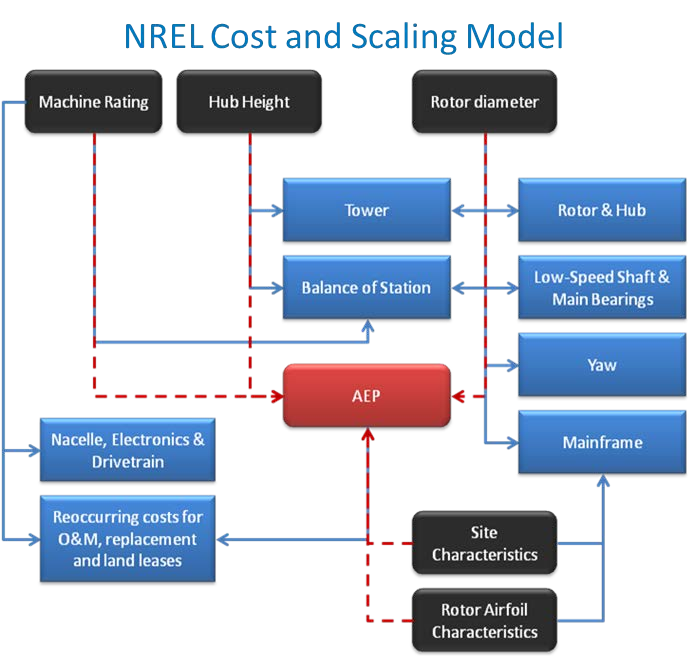
\includegraphics[width=5.5in]{NRELCSM.pdf}
\caption{NREL Cost and Scaling Model Key Input-Output Relationships.}\label{theory:nrelcsm}\end{figure}

The resulting NREL Cost and Scaling Model allows for a variety of interesting analyses including scaling of conventional technology from under a MW to 5 MW+, assessing impact of trends in input factors for materials and labor on wind plant cost of energy, etc.  However, it does not preserve the underlying engineering relationships of the original Sunderland model and thus loses some fidelity of assessing how design changes may impact system costs.

This model directly implements the full wind plant NREL Cost and Scaling Model as described in {[}Fingersh2006{]} with modifications for the drivetrain as described in {[}Maples2010{]}.



\end{document}
